\chapter{Experimenting with Radar-based Gestures (Additional Results)}
\label{app:radar-experiments}

\section{Experiment 2: Gestures Subsets}

\begin{figure}
  \centering
  \begin{subfigure}{.69\linewidth}
      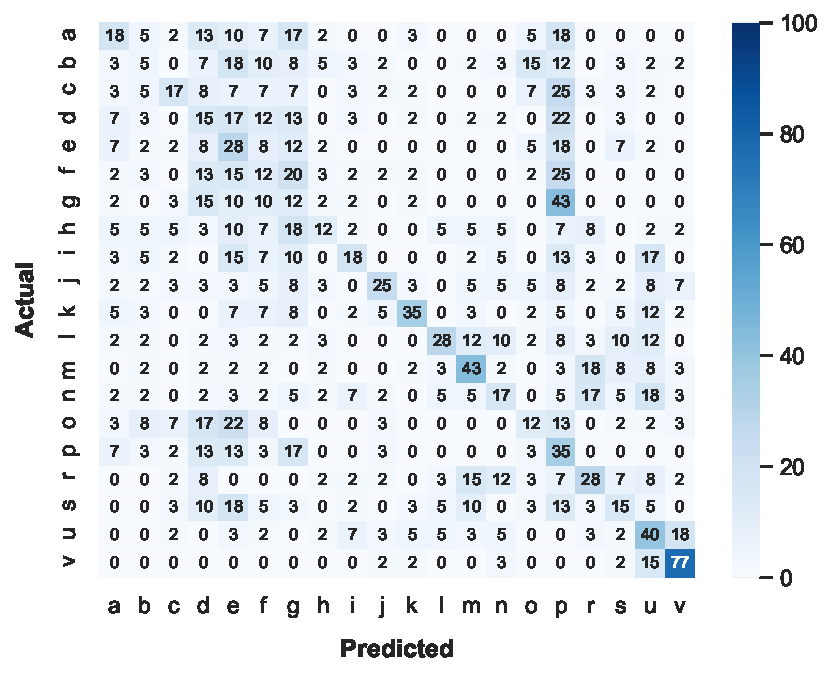
\includegraphics[width=\linewidth]{Figures/RadarExperiments/Datasets/20Gestures/Results/All/UI-time-gating-cm.pdf}
      \vspace{-12pt}
      \caption{Time gating $N{=}38$, \\ $\splitatcommas{AP{=}(1, 2, 3, 6, 8, 9)}$.}
      \vspace{6pt}
      \label{fig:radar-experiments:confusion-exp1-UI-timegating}
  \end{subfigure}
  \begin{subfigure}{.69\linewidth}
      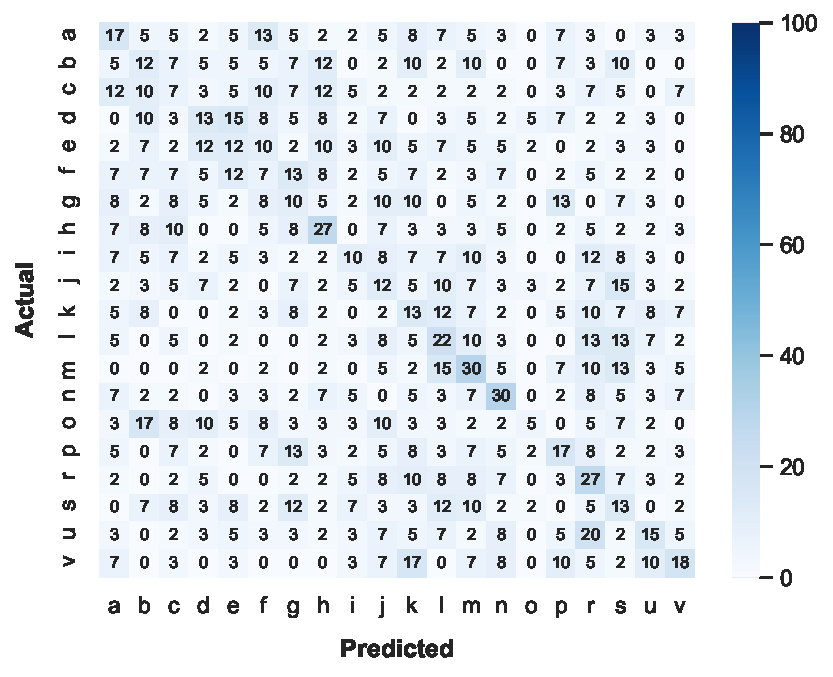
\includegraphics[width=\linewidth]{Figures/RadarExperiments/Datasets/20Gestures/Results/All/UI-filtering-cm.pdf}
      \vspace{-12pt}
      \caption{Filtering $N{=}29$, \\ $\splitatcommas{AP{=}(1, 2, 3, 4, 5, 6, 7, 8, 9, 10, 11, 12)}$.}
      \label{fig:radar-experiments:confusion-exp1-UI-filtering}
  \end{subfigure}
  \caption{Confusion matrices of the best-performing configurations in the user-independent scenario on the complete dataset.}
  \label{fig:radar-experiments:confusion-exp1-UI}
  \vspace{-20pt}
\end{figure}

\begin{figure}
  \centering
  \begin{subfigure}{.69\linewidth}
      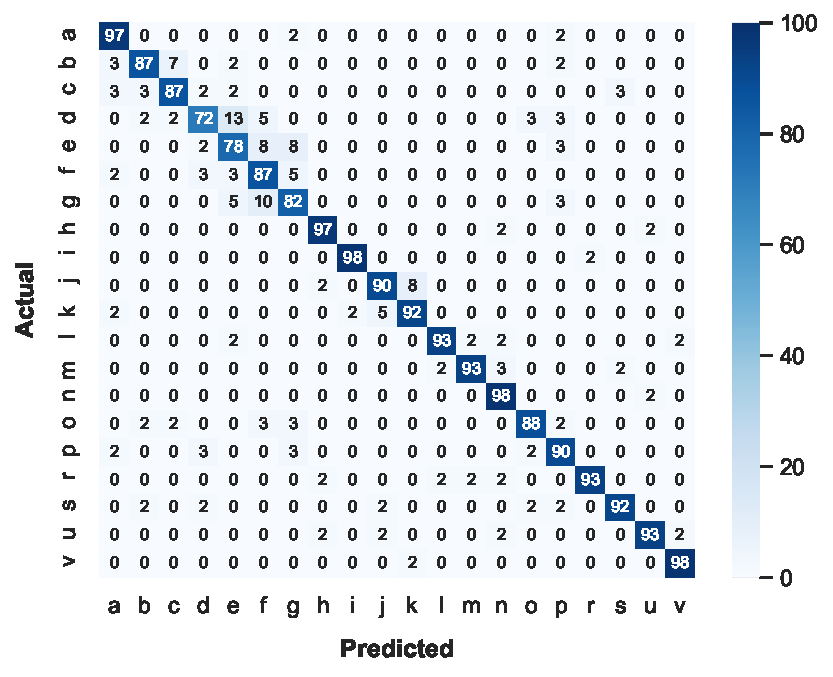
\includegraphics[width=\linewidth]{Figures/RadarExperiments/Datasets/20Gestures/Results/All/Mixed-time-gating-cm.pdf}
      \vspace{-12pt}
      \caption{Time gating $N{=}39$, \\ $\splitatcommas{AP{=}(1, 2, 3, 6, 8, 9)}$.}
      \vspace{6pt}
      \label{fig:radar-experiments:confusion-exp1-Mixed-timegating}
  \end{subfigure}
  \begin{subfigure}{.69\linewidth}
      \includegraphics[width=\linewidth]{Figures/RadarExperiments/Datasets/20Gestures/Results/All/mixed-filtering-cm.pdf}
      \vspace{-12pt}
      \caption{Filtering $N{=}25$, \\ $\splitatcommas{AP{=}(1, 2, 3, 4, 5, 6, 7, 8, 9, 10, 11, 12)}$.}
      \label{fig:radar-experiments:confusion-exp1-Mixed-filtering}
  \end{subfigure}
  \caption{Confusion matrices of the best-performing configurations in the mixed scenario on the complete dataset.}
  \label{fig:radar-experiments:confusion-exp1-Mixed}
  \vspace{-20pt}
\end{figure}

\FloatBarrier

\section{Experiment 3: Gestures through Materials}
% PVC
\begin{figure}[ht]
  \begin{subfigure}{.49\textwidth}
    \centering
    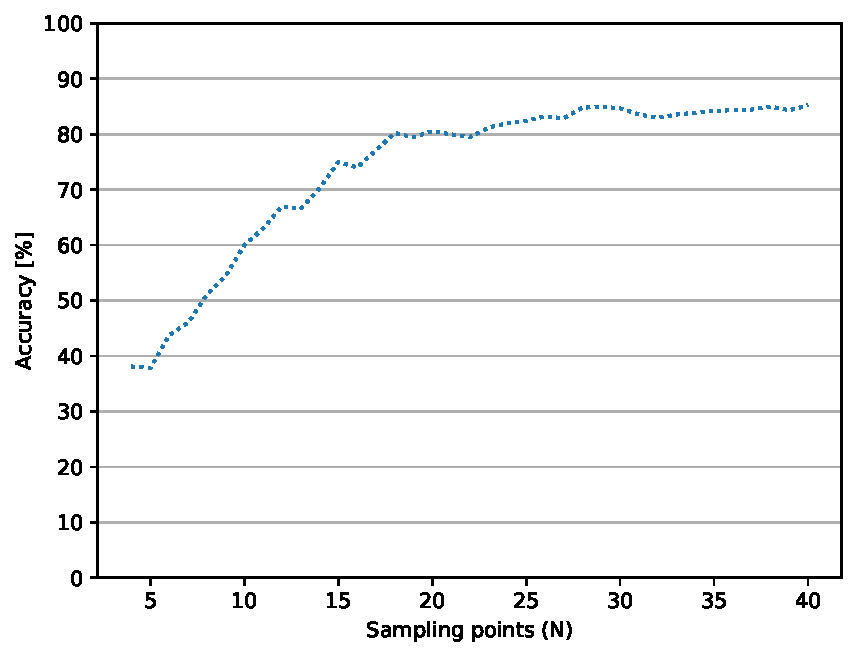
\includegraphics[width=.99\linewidth]{Figures/RadarExperiments/Datasets/ThroughMaterials/PVC/samples-timegating-ud.pdf}
    \vspace{-15pt}
    \captionsetup{width=.99\linewidth}
    \caption{Time gating UD \\ $\splitatcommas{AP{=}(4, 5, 7, 10, 11, 12)}$.}
    \label{fig:radar-experiments:through-materials:pvc-samples:timegating-ud}
  \end{subfigure}
  \begin{subfigure}{.49\textwidth}
    \centering
    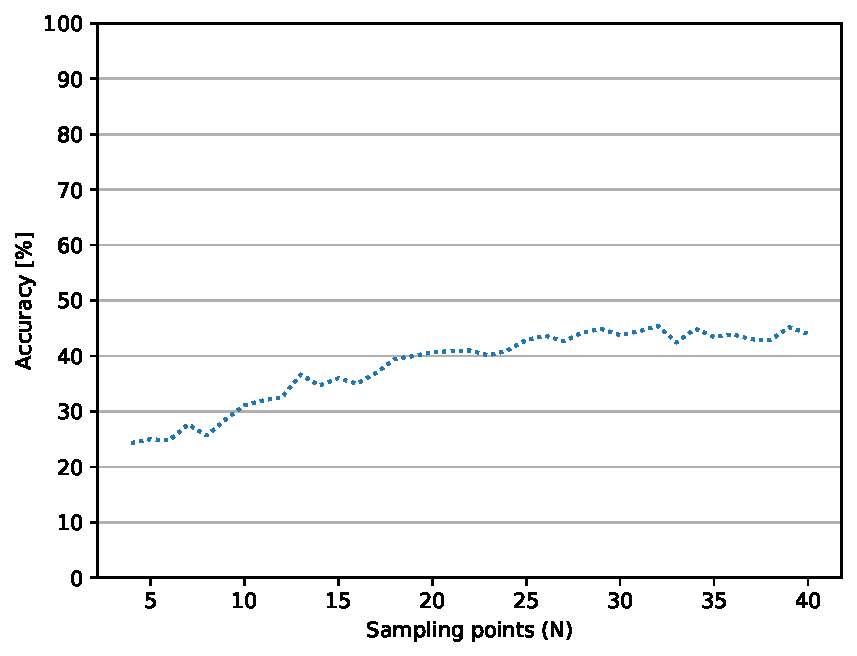
\includegraphics[width=.99\linewidth]{Figures/RadarExperiments/Datasets/ThroughMaterials/PVC/samples-filtering-ud.pdf}  
    \vspace{-15pt}
    \captionsetup{width=.99\linewidth}
    \caption{Filtering UD \\ $\splitatcommas{AP{=}(1, 2, 3, 4, 5, 6, 7, 8, 9, 10, 11, 12)}$.}
    \label{fig:radar-experiments:through-materials:pvc-samples:filtering-ud}
  \end{subfigure}

  \begin{subfigure}{.49\textwidth}
    \centering
    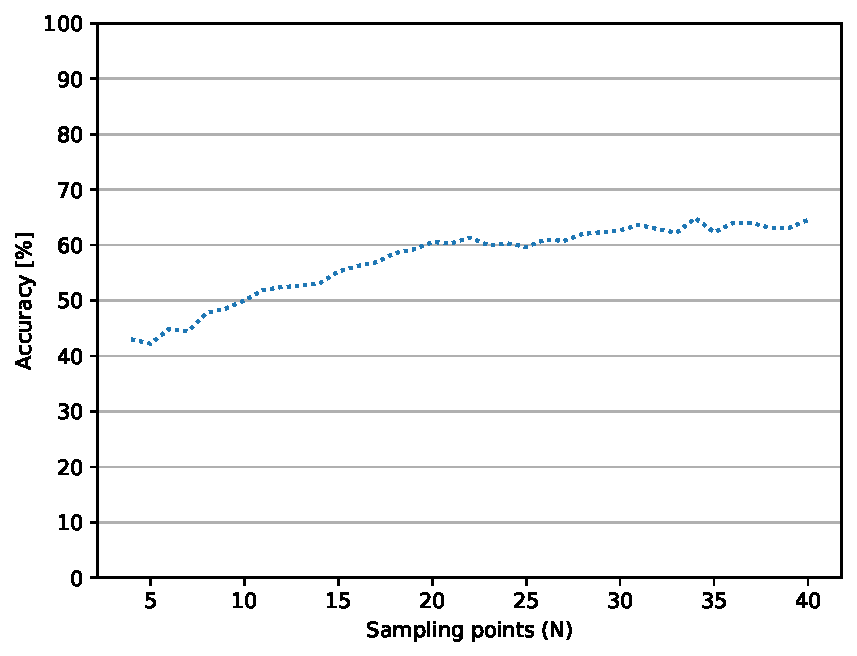
\includegraphics[width=.99\linewidth]{Figures/RadarExperiments/Datasets/ThroughMaterials/PVC/samples-timegating-ui.pdf}
    \vspace{-15pt}
    \captionsetup{width=.99\linewidth}
    \caption{Time gating UI \\ $\splitatcommas{AP{=}(4, 5, 7, 10, 11, 12)}$.}
    \label{fig:radar-experiments:through-materials:pvc-samples:timegating-ui}
  \end{subfigure}
  \begin{subfigure}{.49\textwidth}
    \centering
    \includegraphics[width=.99\linewidth]{Figures/RadarExperiments/Datasets/ThroughMaterials/PVC/samples-filtering-ui.pdf}  
    \vspace{-15pt}
    \captionsetup{width=.99\linewidth}
    \caption{Filtering UI \\ $\splitatcommas{AP{=}(1, 2, 3, 6, 8, 9)}$.}
    \label{fig:radar-experiments:through-materials:pvc-samples:filtering-ui}
  \end{subfigure}

  \vspace{-6pt}
  \caption{The accuracy of Jackknife with respect to the number of sampling points for the best performing set of antenna pairs when using PVC data for training and testing in a user-dependent (top) and user-independent scenario (bottom).}
  \label{fig:radar-experiments:through-materials:pvc-samples}
\end{figure}

\begin{figure}[ht]
  \begin{subfigure}{.49\textwidth}
    \centering
    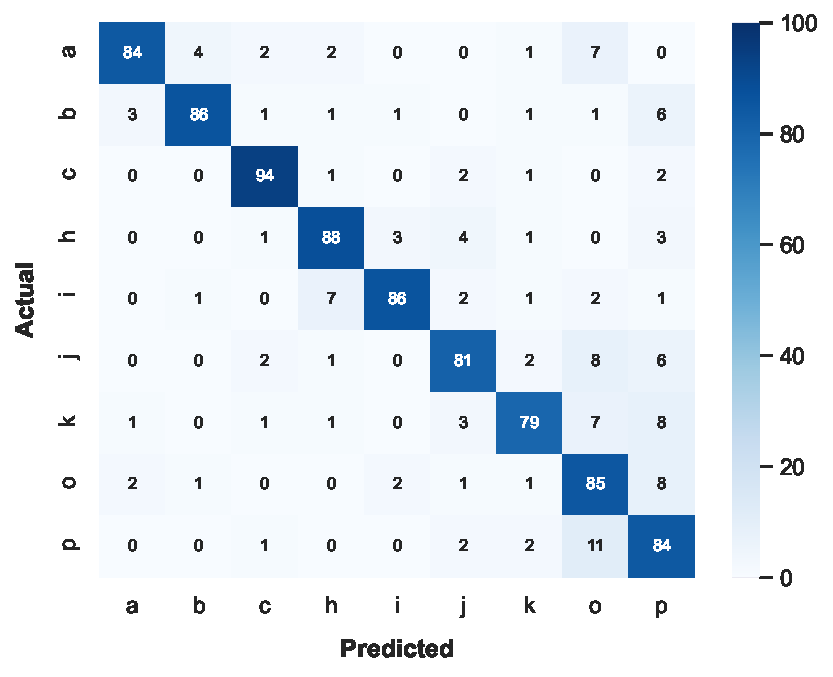
\includegraphics[width=.99\linewidth]{Figures/RadarExperiments/Datasets/ThroughMaterials/PVC/confusion-timegating-ud.pdf}
    \vspace{-15pt}
    \captionsetup{width=.99\linewidth}
    \caption{Time gating UD $N{=}40$, \\ $\splitatcommas{AP{=}(4, 5, 7, 10, 11, 12)}$.}
    \label{fig:radar-experiments:through-materials:pvc-confusion:timegating-ud}
  \end{subfigure}
  \begin{subfigure}{.49\textwidth}
    \centering
    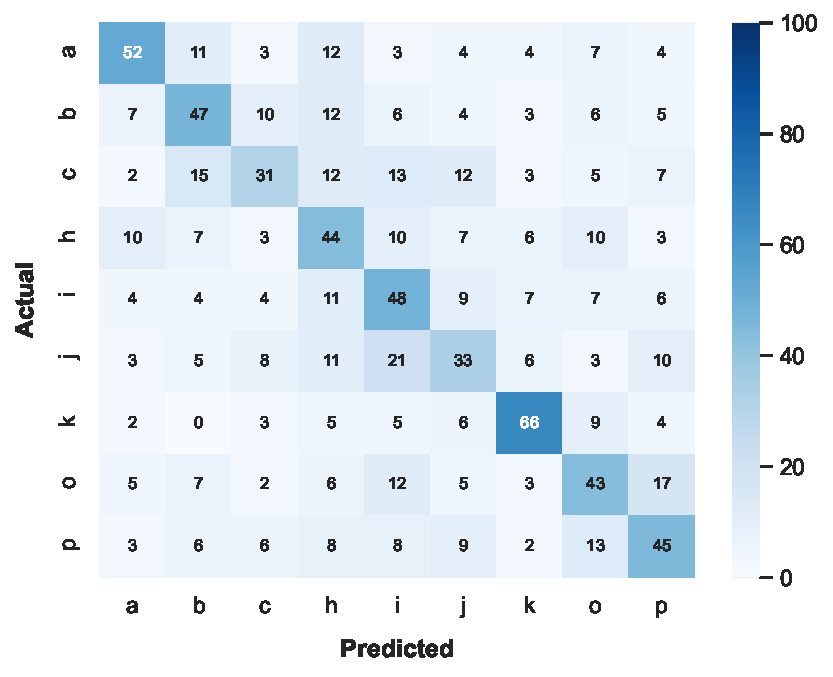
\includegraphics[width=.99\linewidth]{Figures/RadarExperiments/Datasets/ThroughMaterials/PVC/confusion-filtering-ud.pdf}
    \vspace{-15pt}
    \captionsetup{width=.99\linewidth}
    \caption{Filtering UD $N{=}32$, \\ $\splitatcommas{AP{=}(1, 2, 3, 4, 5, 6, 7, 8, 9, 10, 11, 12)}$.}
    \label{fig:radar-experiments:through-materials:pvc-confusion:filtering-ud}
  \end{subfigure}
  
  \begin{subfigure}{.49\textwidth}
    \centering
    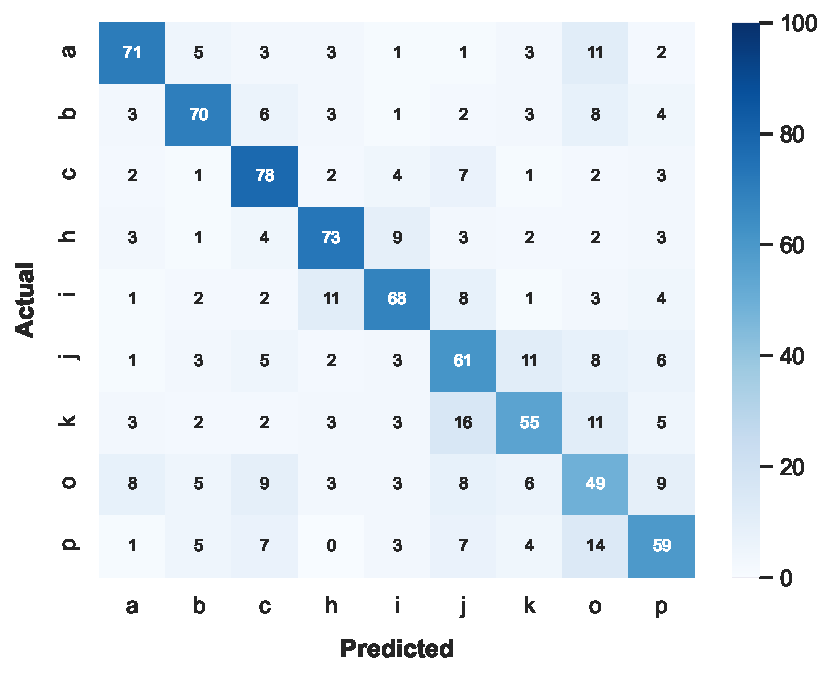
\includegraphics[width=.99\linewidth]{Figures/RadarExperiments/Datasets/ThroughMaterials/PVC/confusion-timegating-ui.pdf}  
    \vspace{-15pt}
    \captionsetup{width=.99\linewidth}
    \caption{Time gating UI $N{=}34$, \\ $\splitatcommas{AP{=}(4, 5, 7, 10, 11, 12)}$.}
    \label{fig:radar-experiments:through-materials:pvc-confusion:timegating-ui}
  \end{subfigure}
  \begin{subfigure}{.49\textwidth}
    \centering
    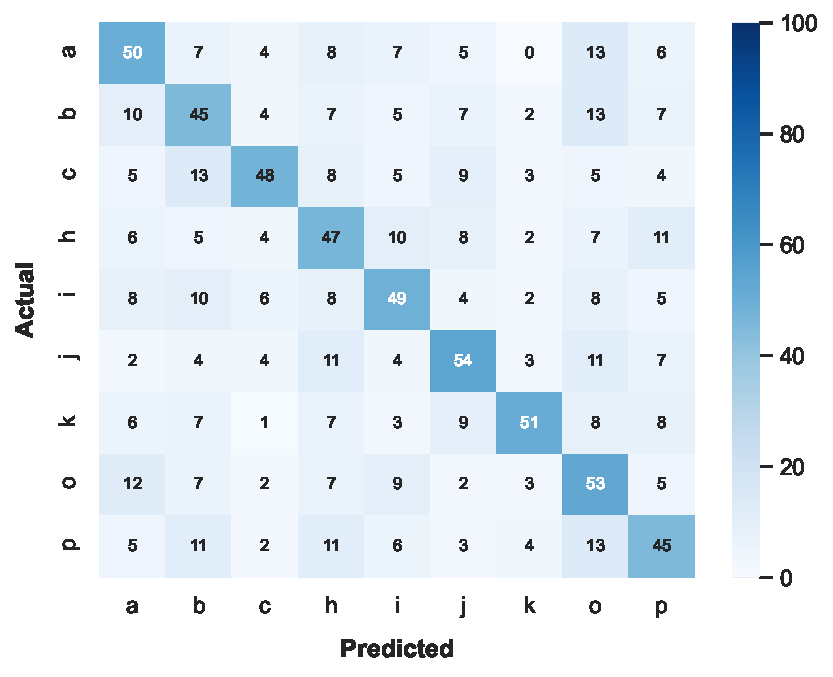
\includegraphics[width=.99\linewidth]{Figures/RadarExperiments/Datasets/ThroughMaterials/PVC/confusion-filtering-ui.pdf}
    \vspace{-15pt}
    \captionsetup{width=.99\linewidth}
    \caption{Filtering UI $N{=}38$, \\ $\splitatcommas{AP{=}(1, 2, 3, 6, 8, 9)}$.}
    \label{fig:radar-experiments:through-materials:pvc-confusion:filtering-ui}
  \end{subfigure}

  \vspace{-6pt}
    \caption{Normalized confusion matrices for the best configuration at two stages of the pipeline in user-dependent (top) and user-independent scenarios (bottom) when using PVC data for training and testing. The values in each cell are represented as percentages.}
    \label{fig:radar-experiments:through-materials:pvc-confusion}
\end{figure}



% GLASS
\begin{figure}[ht]
  \begin{subfigure}{.49\textwidth}
    \centering
    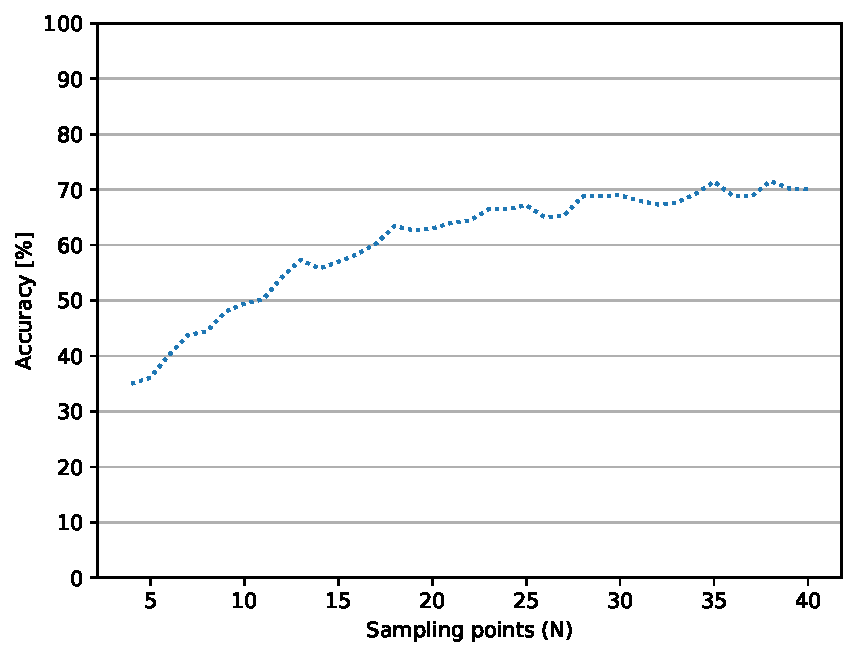
\includegraphics[width=.99\linewidth]{Figures/RadarExperiments/Datasets/ThroughMaterials/Glass/samples-timegating-ud.pdf}
    \vspace{-15pt}
    \captionsetup{width=.99\linewidth}
    \caption{Time gating UD \\ $\splitatcommas{AP{=}(1, 2, 3, 6, 8, 9)}$.}
    \label{fig:radar-experiments:through-materials:glass-samples:timegating-ud}
  \end{subfigure}
  \begin{subfigure}{.49\textwidth}
    \centering
    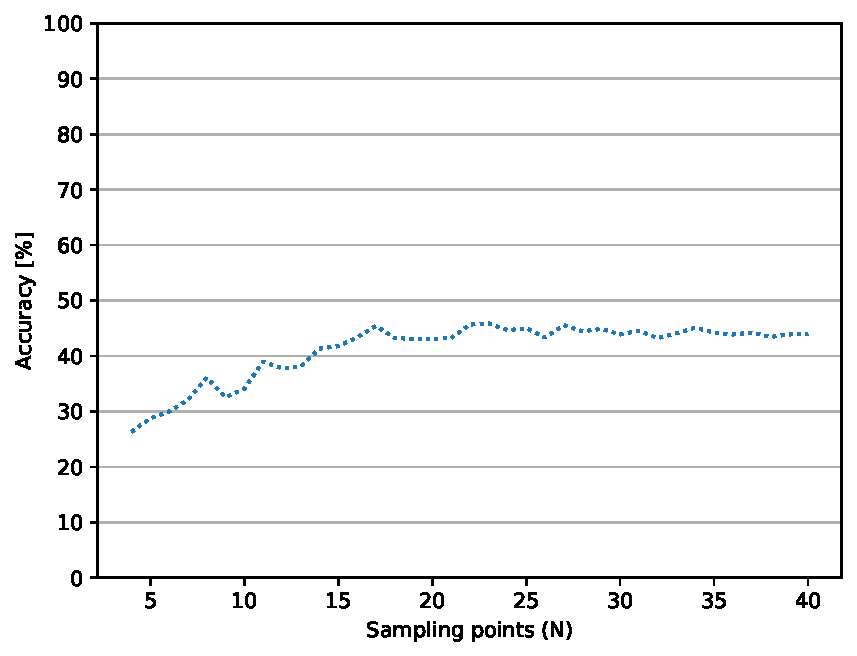
\includegraphics[width=.99\linewidth]{Figures/RadarExperiments/Datasets/ThroughMaterials/Glass/samples-filtering-ud.pdf}  
    \vspace{-15pt}
    \captionsetup{width=.99\linewidth}
    \caption{Filtering UD \\ $\splitatcommas{AP{=}(1, 2, 3, 4, 5, 6, 7, 8, 9, 10, 11, 12)}$.}
    \label{fig:radar-experiments:through-materials:glass-samples:filtering-ud}
  \end{subfigure}

  \begin{subfigure}{.49\textwidth}
    \centering
    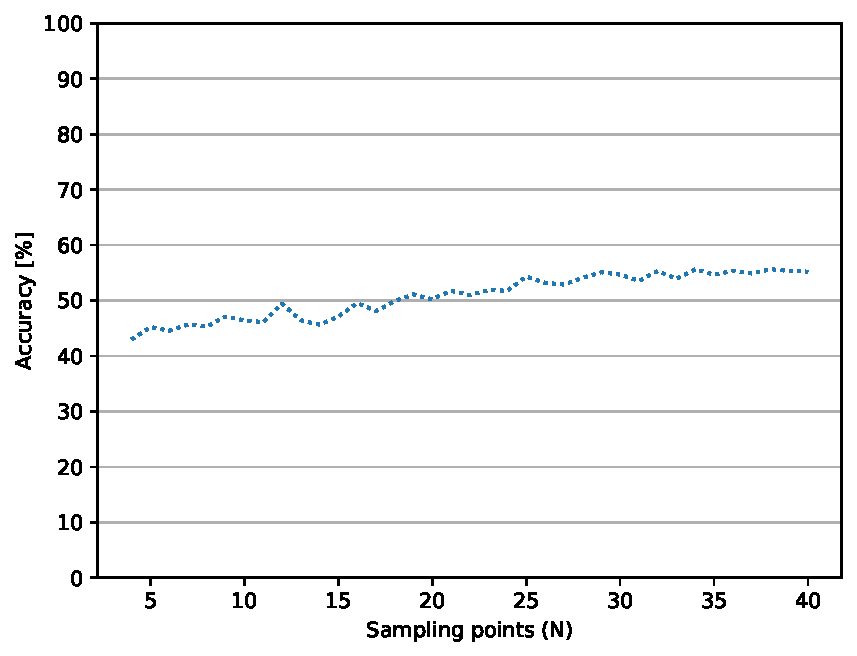
\includegraphics[width=.99\linewidth]{Figures/RadarExperiments/Datasets/ThroughMaterials/Glass/samples-timegating-ui.pdf}
    \vspace{-15pt}
    \captionsetup{width=.99\linewidth}
    \caption{Time gating UI \\ $\splitatcommas{AP{=}(1, 2, 3, 6, 8, 9)}$.}
    \label{fig:radar-experiments:through-materials:glass-samples:timegating-ui}
  \end{subfigure}
  \begin{subfigure}{.49\textwidth}
    \centering
    \includegraphics[width=.99\linewidth]{Figures/RadarExperiments/Datasets/ThroughMaterials/Glass/samples-filtering-ui.pdf}  
    \vspace{-15pt}
    \captionsetup{width=.99\linewidth}
    \caption{Filtering UI \\ $\splitatcommas{AP{=}(1, 2, 3, 4, 5, 6, 7, 8, 9, 10, 11, 12)}$.}
    \label{fig:radar-experiments:through-materials:glass-samples:filtering-ui}
  \end{subfigure}

  \vspace{-6pt}
  \caption{The accuracy of Jackknife with respect to the number of sampling points for the best performing set of antenna pairs when using glass data for training and testing in a user-dependent (top) and user-independent scenario (bottom).}
  \label{fig:radar-experiments:through-materials:glass-samples}
\end{figure}

\begin{figure}[ht]
  \begin{subfigure}{.49\textwidth}
    \centering
    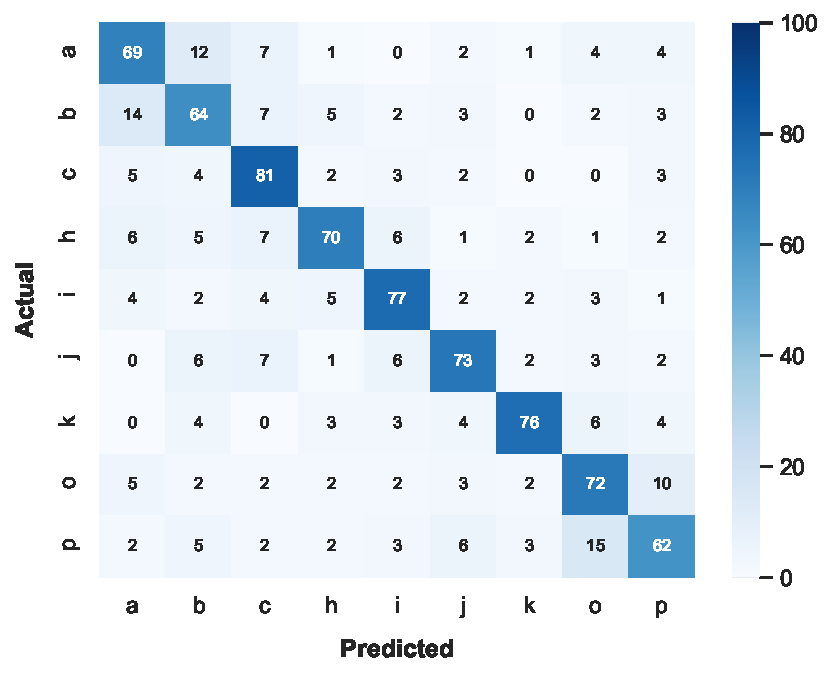
\includegraphics[width=.99\linewidth]{Figures/RadarExperiments/Datasets/ThroughMaterials/Glass/confusion-timegating-ud.pdf}
    \vspace{-15pt}
    \captionsetup{width=.99\linewidth}
    \caption{Time gating UD $N{=}38$, \\ $\splitatcommas{AP{=}(1, 2, 3, 6, 8, 9)}$.}
    \label{fig:radar-experiments:through-materials:glass-confusion:timegating-ud}
  \end{subfigure}
  \begin{subfigure}{.49\textwidth}
    \centering
    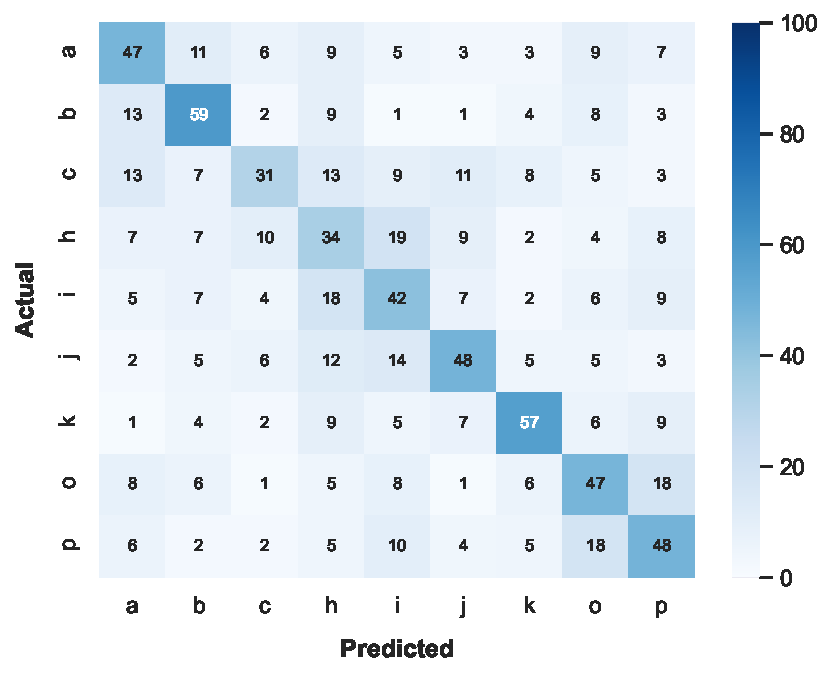
\includegraphics[width=.99\linewidth]{Figures/RadarExperiments/Datasets/ThroughMaterials/Glass/confusion-filtering-ud.pdf}
    \vspace{-15pt}
    \captionsetup{width=.99\linewidth}
    \caption{Filtering UD $N{=}23$, \\ $\splitatcommas{AP{=}(1, 2, 3, 4, 5, 6, 7, 8, 9, 10, 11, 12)}$.}
    \label{fig:radar-experiments:through-materials:glass-confusion:filtering-ud}
  \end{subfigure}

  \begin{subfigure}{.49\textwidth}
    \centering
    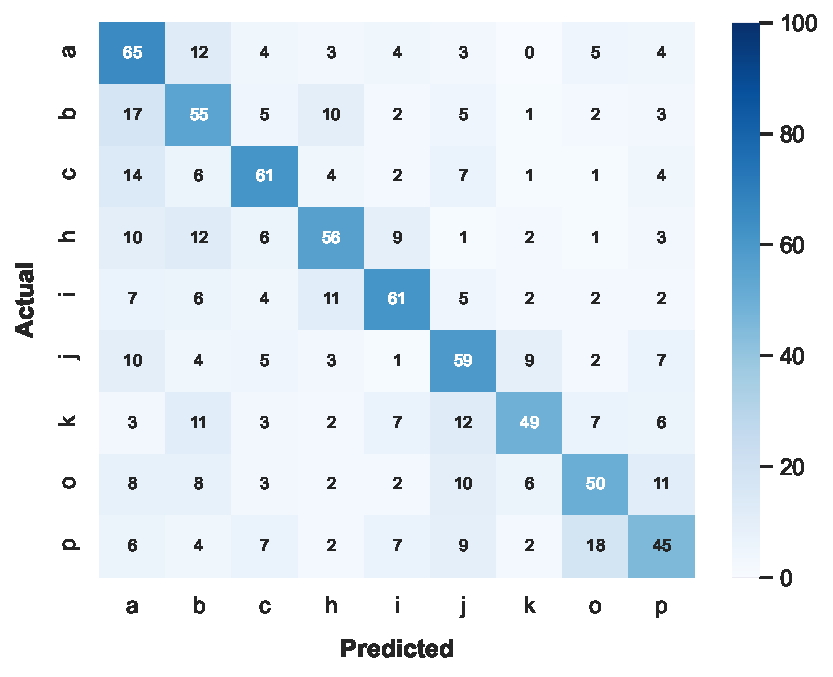
\includegraphics[width=.99\linewidth]{Figures/RadarExperiments/Datasets/ThroughMaterials/Glass/confusion-timegating-ui.pdf}  
    \vspace{-15pt}
    \captionsetup{width=.99\linewidth}
    \caption{Time gating UI $N{=}34$, \\ $\splitatcommas{AP{=}(1, 2, 3, 6, 8, 9)}$.}
    \label{fig:radar-experiments:through-materials:glass-confusion:timegating-ui}
  \end{subfigure}
  \begin{subfigure}{.49\textwidth}
    \centering
    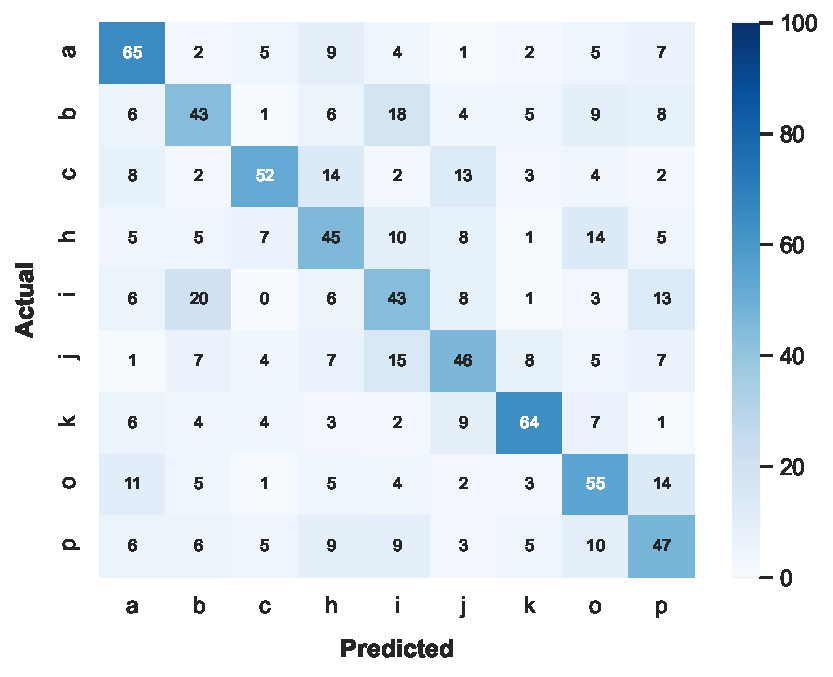
\includegraphics[width=.99\linewidth]{Figures/RadarExperiments/Datasets/ThroughMaterials/Glass/confusion-filtering-ui.pdf}
    \vspace{-15pt}
    \captionsetup{width=.99\linewidth}
    \caption{Filtering UI $N{=}36$, \\ $\splitatcommas{AP{=}(1, 2, 3, 4, 5, 6, 7, 8, 9, 10, 11, 12)}$.}
    \label{fig:radar-experiments:through-materials:glass-confusion:filtering-ui}
  \end{subfigure}

  \vspace{-6pt}
    \caption{Normalized confusion matrices for the best configuration at two stages of the pipeline in user-dependent (top) and user-independent scenarios (bottom) when using glass data for training and testing. The values in each cell are represented as percentages.}
    \label{fig:radar-experiments:through-materials:glass-confusion}
\end{figure}





% PVC+WOOD
\begin{figure}[ht]
  \begin{subfigure}{.49\textwidth}
    \centering
    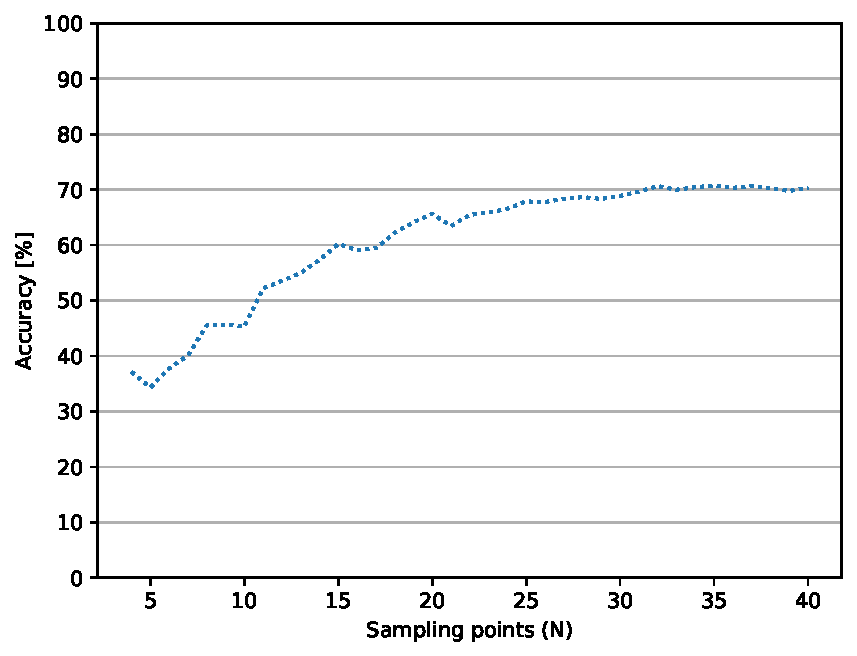
\includegraphics[width=.99\linewidth]{Figures/RadarExperiments/Datasets/ThroughMaterials/PVC+Wood/samples-timegating-ud.pdf}
    \vspace{-15pt}
    \captionsetup{width=.99\linewidth}
    \caption{Time gating \\ $\splitatcommas{AP{=}(4, 5, 7, 10, 11, 12)}$.}
    \label{fig:radar-experiments:through-materials:pvc-wood-samples:timegating-ud}
  \end{subfigure}
  \begin{subfigure}{.49\textwidth}
    \centering
    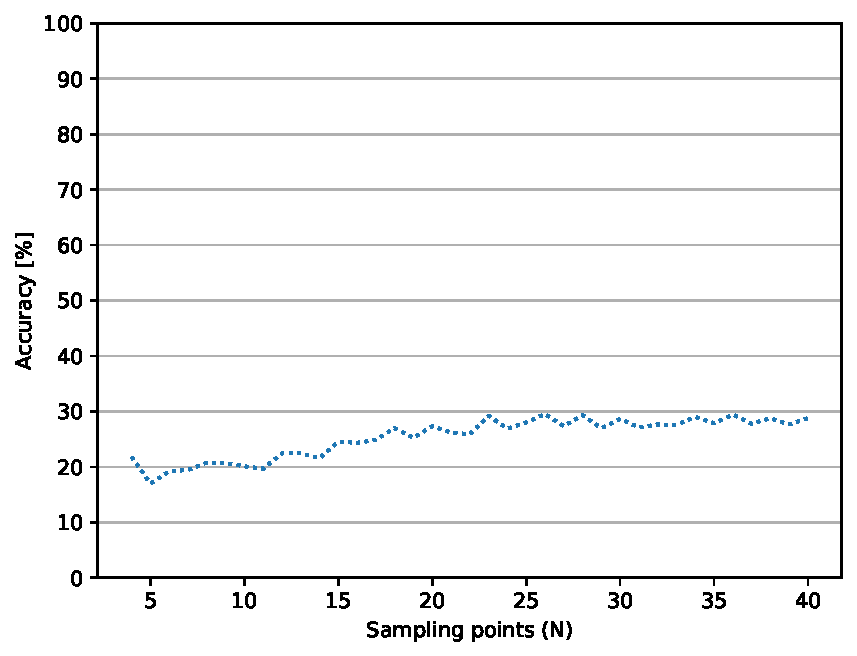
\includegraphics[width=.99\linewidth]{Figures/RadarExperiments/Datasets/ThroughMaterials/PVC+Wood/samples-filtering-ud.pdf}  
    \vspace{-15pt}
    \captionsetup{width=.99\linewidth}
    \caption{Filtering \\ $\splitatcommas{AP{=}(1, 2, 3, 4, 5, 6, 7, 8, 9, 10, 11, 12)}$.}
    \label{fig:radar-experiments:through-materials:pvc-wood-samples:filtering-ud}
  \end{subfigure}

  \vspace{-6pt}
  \caption{The accuracy of Jackknife with respect to the number of sampling points for the best performing set of antenna pairs when using PVC data for training and wood data for testing in a user-dependent scenario.}
  \label{fig:radar-experiments:through-materials:pvc-wood-samples}
\end{figure}

\begin{figure}[ht]
  \begin{subfigure}{.49\textwidth}
    \centering
    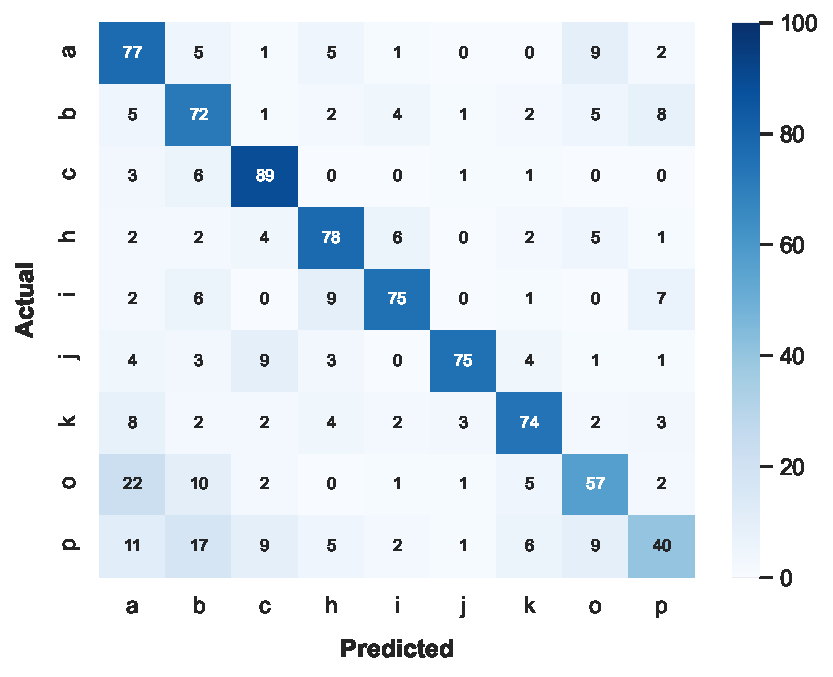
\includegraphics[width=.99\linewidth]{Figures/RadarExperiments/Datasets/ThroughMaterials/PVC+Wood/confusion-timegating-ud.pdf}
    \vspace{-15pt}
    \captionsetup{width=.99\linewidth}
    \caption{Time gating $N{=}35$, \\ $\splitatcommas{AP{=}(4, 5, 7, 10, 11, 12)}$.}
    \label{fig:radar-experiments:through-materials:pvc-wood-confusion:timegating-ud}
  \end{subfigure}
  \begin{subfigure}{.49\textwidth}
    \centering
    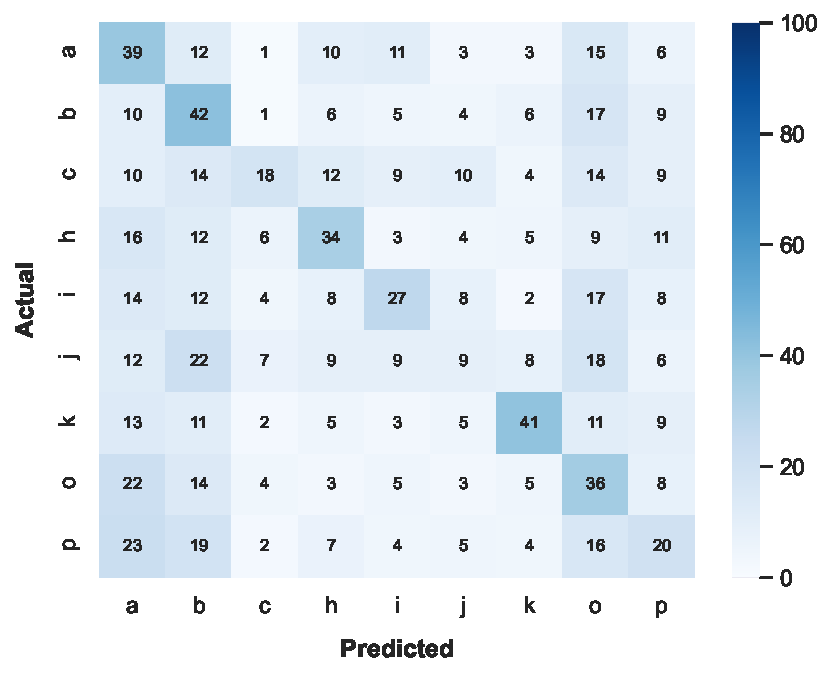
\includegraphics[width=.99\linewidth]{Figures/RadarExperiments/Datasets/ThroughMaterials/PVC+Wood/confusion-filtering-ud.pdf}
    \vspace{-15pt}
    \captionsetup{width=.99\linewidth}
    \caption{Filtering $N{=}26$, \\ $\splitatcommas{AP{=}(1, 2, 3, 4, 5, 6, 7, 8, 9, 10, 11, 12)}$.}
    \label{fig:radar-experiments:through-materials:pvc-wood-confusion:filtering-ud}
  \end{subfigure}
  
  \vspace{-6pt}
  \caption{Normalized confusion matrices for the best configuration at two stages of the pipeline in the user-dependent scenario when using PVC data for training and wood data for testing. The values in each cell are represented as percentages.}
  \label{fig:radar-experiments:through-materials:pvc-wood-confusion}
\end{figure}






% WOOD+GLASS
\begin{figure}[ht]
  \begin{subfigure}{.49\textwidth}
    \centering
    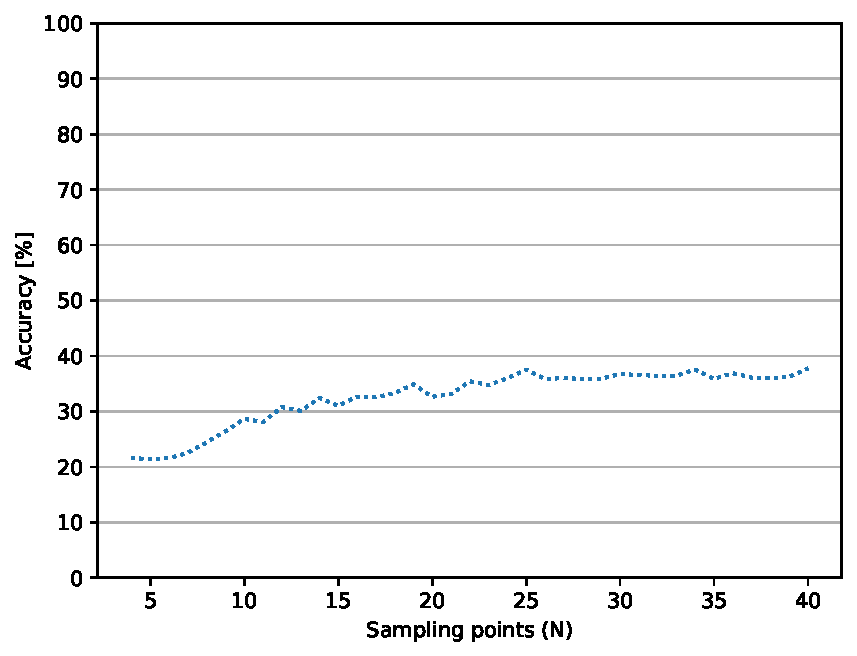
\includegraphics[width=.99\linewidth]{Figures/RadarExperiments/Datasets/ThroughMaterials/Wood+Glass/samples-timegating-ud.pdf}
    \vspace{-5pt}
    \captionsetup{width=.99\linewidth}
    \caption{Time gating \\ $\splitatcommas{AP{=}(1, 2, 3, 6, 8, 9)}$.}
    \label{fig:radar-experiments:through-materials:wood-glass-samples:timegating-ud}
  \end{subfigure}
  \begin{subfigure}{.49\textwidth}
    \centering
    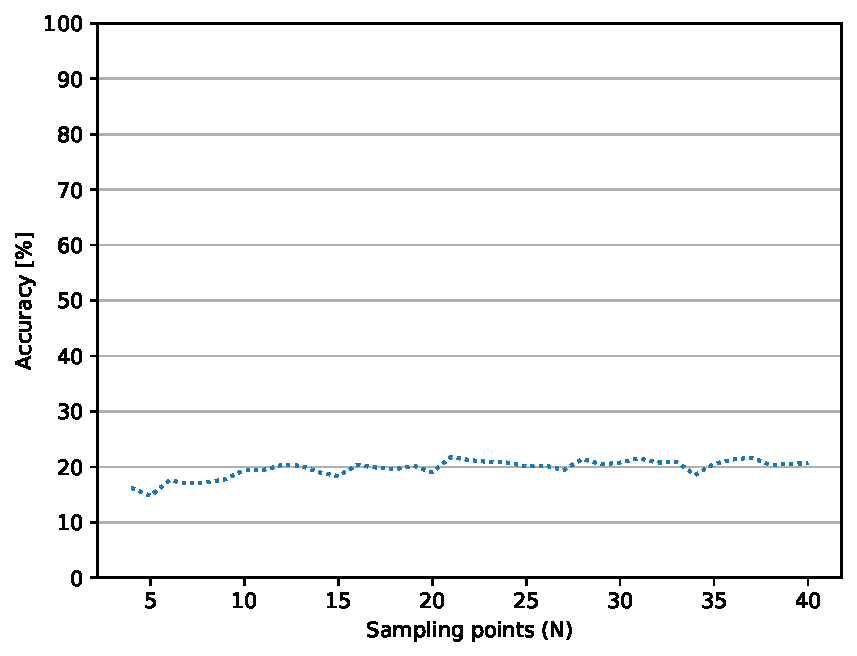
\includegraphics[width=.99\linewidth]{Figures/RadarExperiments/Datasets/ThroughMaterials/Wood+Glass/samples-filtering-ud.pdf}  
    \vspace{-5pt}
    \captionsetup{width=.99\linewidth}
    \caption{Filtering \\ $\splitatcommas{AP{=}(1, 2, 3, 6, 8, 9)}$.}
    \label{fig:radar-experiments:through-materials:wood-glass-samples:filtering-ud}
  \end{subfigure}

  \vspace{-6pt}
  \caption{The accuracy of Jackknife with respect to the number of sampling points for the best performing set of antenna pairs when using wood data for training and glass data for testing in a user-dependent scenario.}
  \label{fig:radar-experiments:through-materials:wood-glass-samples}
\end{figure}

\begin{figure}[ht]
  \begin{subfigure}{.49\textwidth}
    \centering
    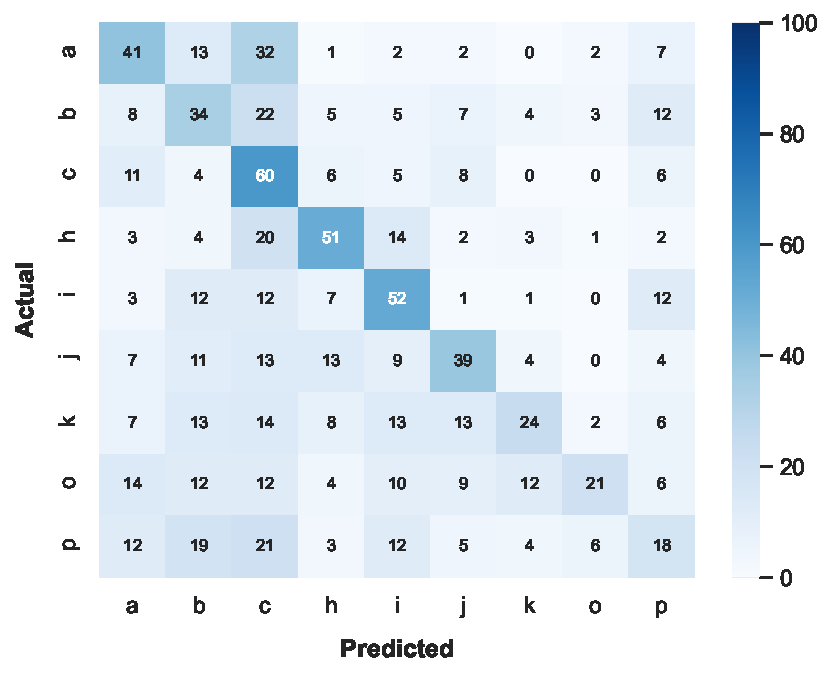
\includegraphics[width=.99\linewidth]{Figures/RadarExperiments/Datasets/ThroughMaterials/Wood+Glass/confusion-timegating-ud.pdf}
    \vspace{-5pt}
    \captionsetup{width=.99\linewidth}
    \caption{Time gating $N{=}40$, \\ $\splitatcommas{AP{=}(1, 2, 3, 6, 8, 9)}$.}
    \label{fig:radar-experiments:through-materials:wood-glass-confusion:timegating-ud}
  \end{subfigure}
  \begin{subfigure}{.49\textwidth}
    \centering
    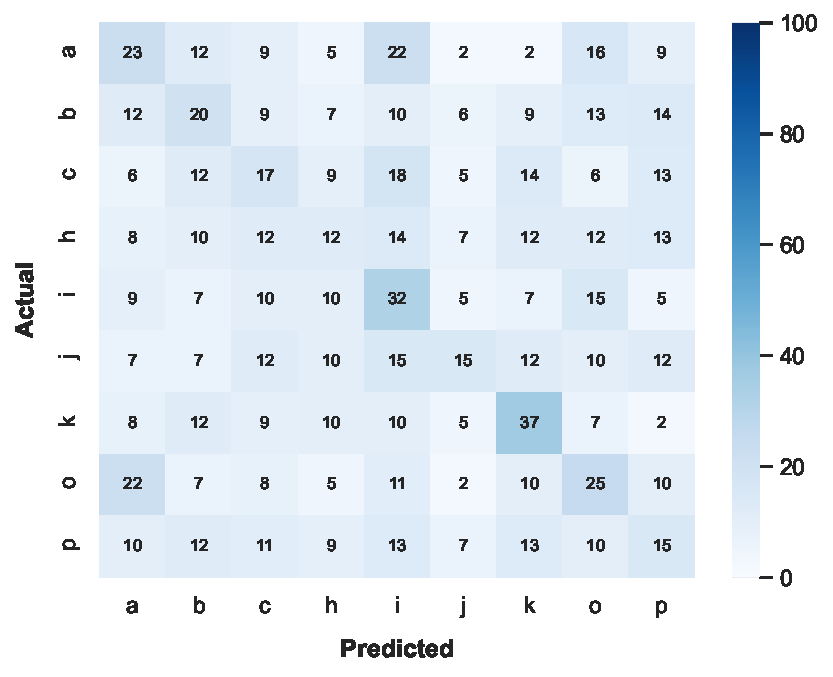
\includegraphics[width=.99\linewidth]{Figures/RadarExperiments/Datasets/ThroughMaterials/Wood+Glass/confusion-filtering-ud.pdf}
    \vspace{-5pt}
    \captionsetup{width=.99\linewidth}
    \caption{Filtering $N{=}21$, \\ $\splitatcommas{AP{=}(1, 2, 3, 6, 8, 9)}$.}
    \label{fig:radar-experiments:through-materials:wood-glass-confusion:filtering-ud}
  \end{subfigure}
  
  \vspace{-6pt}
  \caption{Normalized confusion matrices for the best configuration at two stages of the pipeline in the user-dependent scenario when using wood data for training and glass data for testing. The values in each cell are represented as percentages.}
  \label{fig:radar-experiments:through-materials:wood-glass-confusion}
\end{figure}


% GLASS+WOOD
\begin{figure}[ht]
  \begin{subfigure}{.49\textwidth}
    \centering
    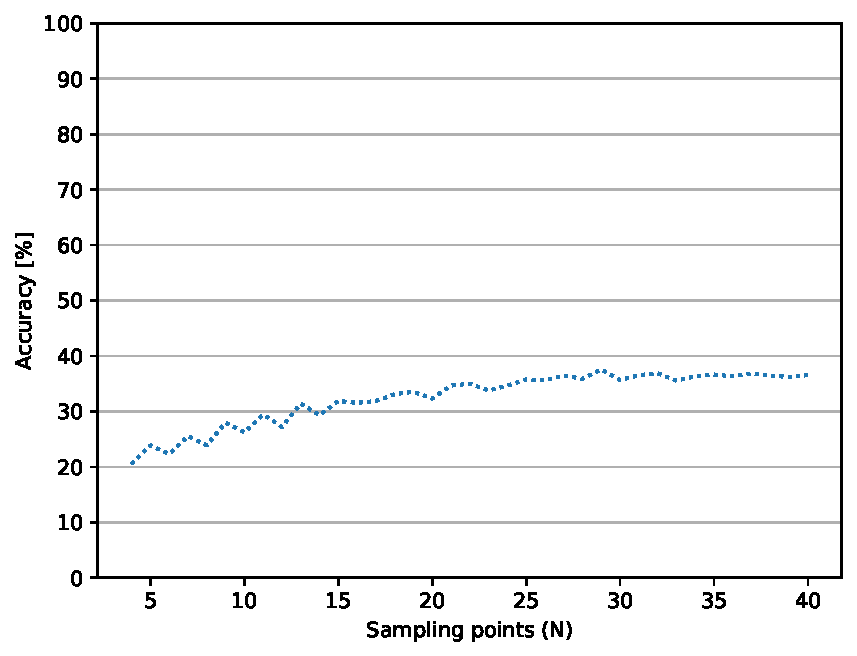
\includegraphics[width=.99\linewidth]{Figures/RadarExperiments/Datasets/ThroughMaterials/Glass+Wood/samples-timegating-ud.pdf}
    \vspace{-15pt}
    \captionsetup{width=.99\linewidth}
    \caption{Time gating \\ $\splitatcommas{AP{=}(1, 2, 3, 6, 8, 9)}$.}
    \label{fig:radar-experiments:through-materials:glass-wood-samples:timegating-ud}
  \end{subfigure}
  \begin{subfigure}{.49\textwidth}
    \centering
    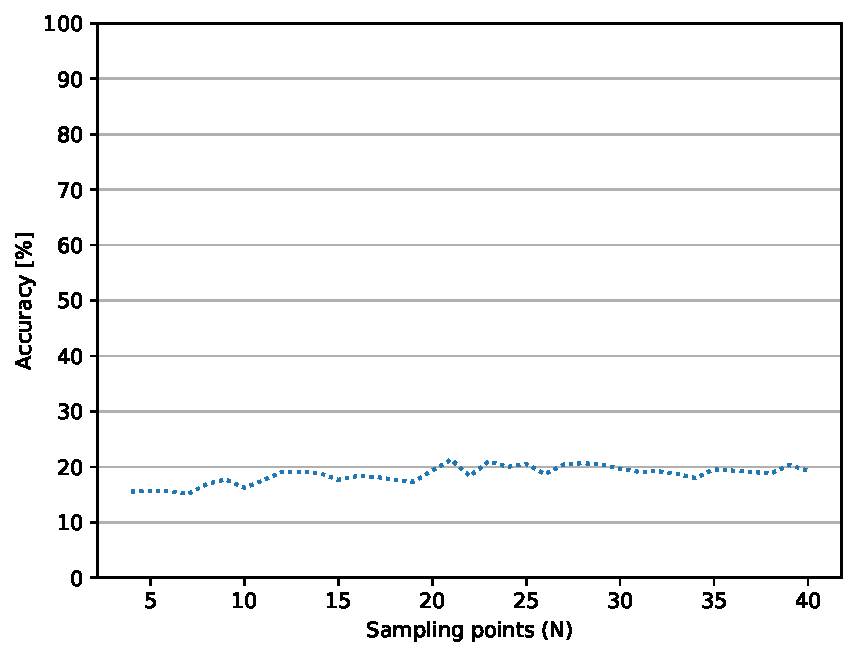
\includegraphics[width=.99\linewidth]{Figures/RadarExperiments/Datasets/ThroughMaterials/Glass+Wood/samples-filtering-ud.pdf}  
    \vspace{-15pt}
    \captionsetup{width=.99\linewidth}
    \caption{Filtering \\ $\splitatcommas{AP{=}(1, 2, 3, 6, 8, 9)}$.}
    \label{fig:radar-experiments:through-materials:glass-wood-samples:filtering-ud}
  \end{subfigure}

  \vspace{-6pt}
  \caption{The accuracy of Jackknife with respect to the number of sampling points for the best performing set of antenna pairs when using glass data for training and wood data for testing in a user-dependent scenario.}
  \label{fig:radar-experiments:through-materials:glass-wood-samples}
\end{figure}

\begin{figure}[ht]
  \begin{subfigure}{.49\textwidth}
      \centering
      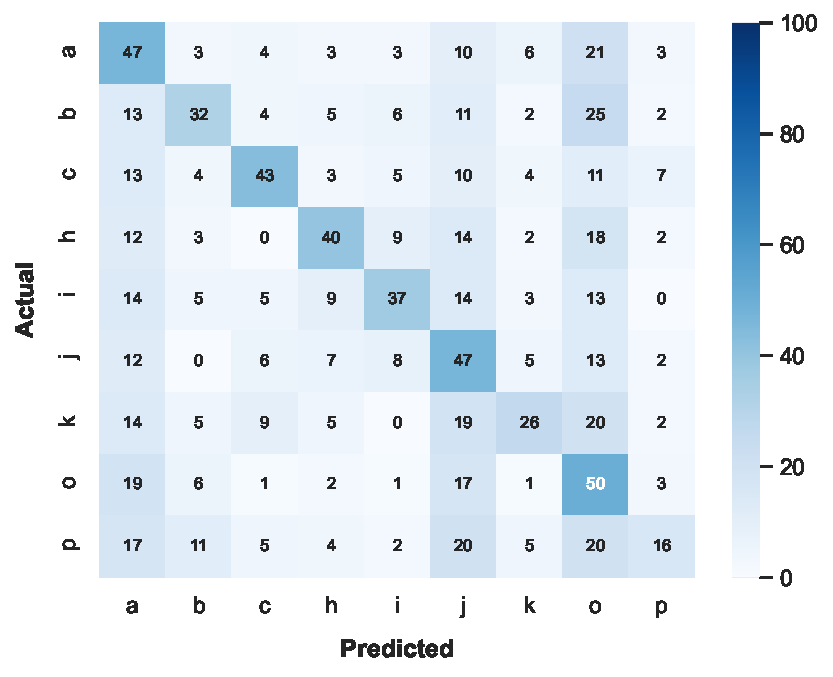
\includegraphics[width=.99\linewidth]{Figures/RadarExperiments/Datasets/ThroughMaterials/Glass+Wood/confusion-timegating-ud.pdf}
      \vspace{-15pt}
      \captionsetup{width=.99\linewidth}
      \caption{Time gating $N{=}29$, \\ $\splitatcommas{AP{=}(1, 2, 3, 6, 8, 9)}$.}
      \label{fig:radar-experiments:through-materials:glass-wood-confusion:timegating-ud}
  \end{subfigure}
  \begin{subfigure}{.49\textwidth}
      \centering
      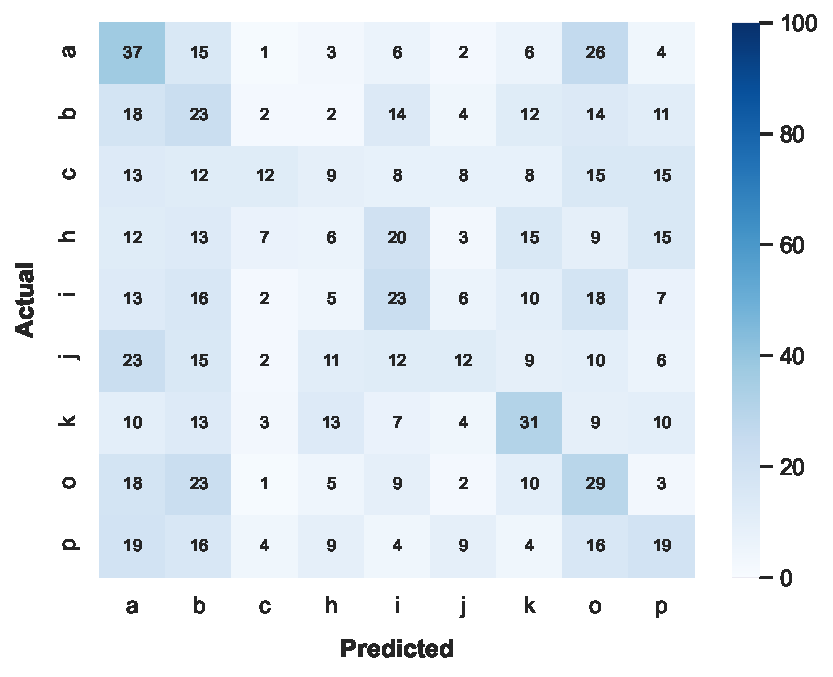
\includegraphics[width=.99\linewidth]{Figures/RadarExperiments/Datasets/ThroughMaterials/Glass+Wood/confusion-filtering-ud.pdf}
      \vspace{-15pt}
      \captionsetup{width=.99\linewidth}
      \caption{Filtering $N{=}21$, \\ $\splitatcommas{AP{=}(1, 2, 3, 6, 8, 9)}$.}
      \label{fig:radar-experiments:through-materials:glass-wood-confusion:filtering-ud}
  \end{subfigure}
  
  \vspace{-6pt}
  \caption{Normalized confusion matrices for the best configuration at two stages of the pipeline in the user-dependent scenario when using glass data for training and wood data for testing. The values in each cell are represented as percentages.}
  \label{fig:radar-experiments:through-materials:glass-wood-confusion}
\end{figure}




% PVC+GLASS
\begin{figure}[ht]
  \begin{subfigure}{.49\textwidth}
    \centering
    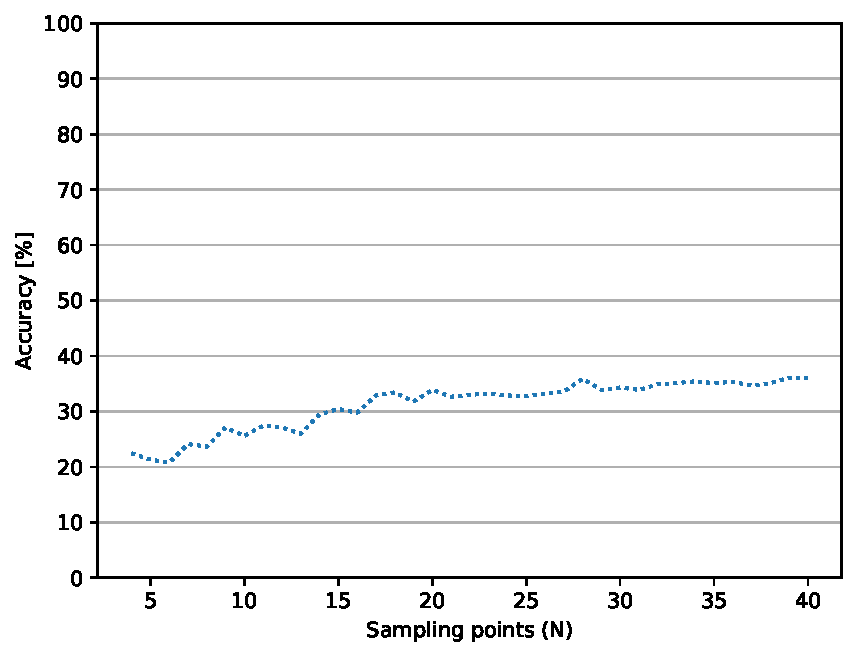
\includegraphics[width=.99\linewidth]{Figures/RadarExperiments/Datasets/ThroughMaterials/PVC+Glass/samples-timegating-ud.pdf}
    \vspace{-15pt}
    \captionsetup{width=.99\linewidth}
    \caption{Time gating \\ $\splitatcommas{AP{=}(1, 2, 3, 6, 8, 9)}$.}
    \label{fig:radar-experiments:through-materials:pvc-glass-samples:timegating-ud}
  \end{subfigure}
  \begin{subfigure}{.49\textwidth}
    \centering
    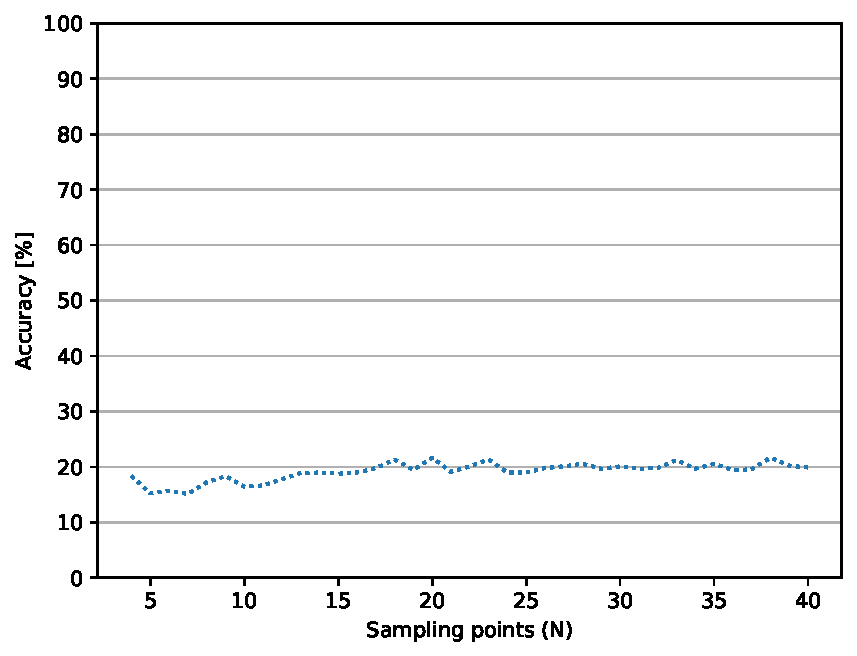
\includegraphics[width=.99\linewidth]{Figures/RadarExperiments/Datasets/ThroughMaterials/PVC+Glass/samples-filtering-ud.pdf}  
    \vspace{-15pt}
    \captionsetup{width=.99\linewidth}
    \caption{Filtering \\ $\splitatcommas{AP{=}(1, 2, 3, 6, 8, 9)}$.}
    \label{fig:radar-experiments:through-materials:pvc-glass-samples:filtering-ud}
  \end{subfigure}

  \vspace{-6pt}
  \caption{The accuracy of Jackknife with respect to the number of sampling points for the best performing set of antenna pairs when using PVC data for training and glass data for testing in a user-dependent scenario.}
  \label{fig:radar-experiments:through-materials:pvc-glass-samples}
\end{figure}

\begin{figure}[ht]
  \begin{subfigure}{.49\textwidth}
      \centering
      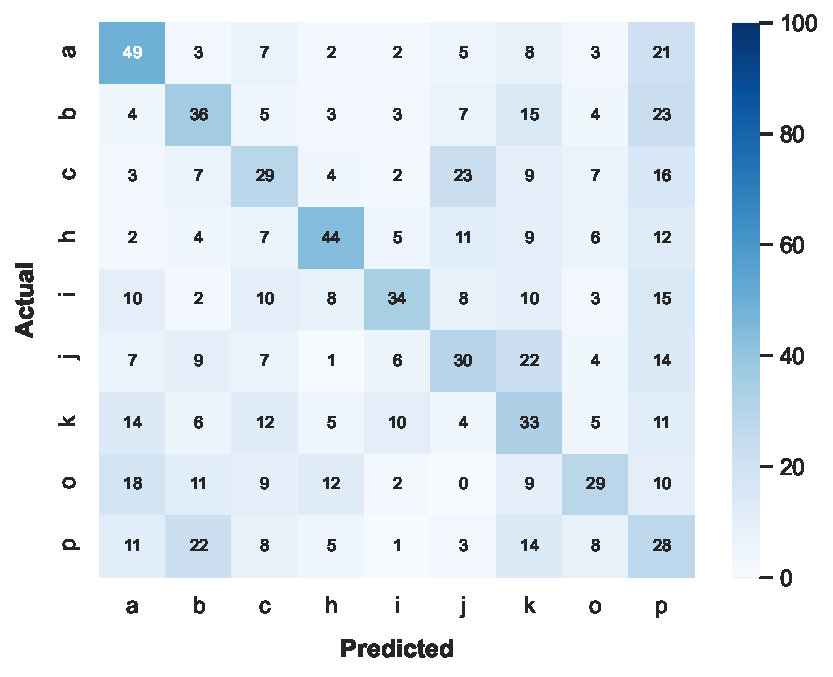
\includegraphics[width=.99\linewidth]{Figures/RadarExperiments/Datasets/ThroughMaterials/PVC+Glass/confusion-timegating-ud.pdf}
      \vspace{-15pt}
      \captionsetup{width=.99\linewidth}
      \caption{Time gating $N{=}37$, \\ $\splitatcommas{AP{=}(1, 2, 3, 6, 8, 9)}$.}
      \label{fig:radar-experiments:through-materials:pvc-glass-confusion:timegating-ud}
  \end{subfigure}
  \begin{subfigure}{.49\textwidth}
      \centering
      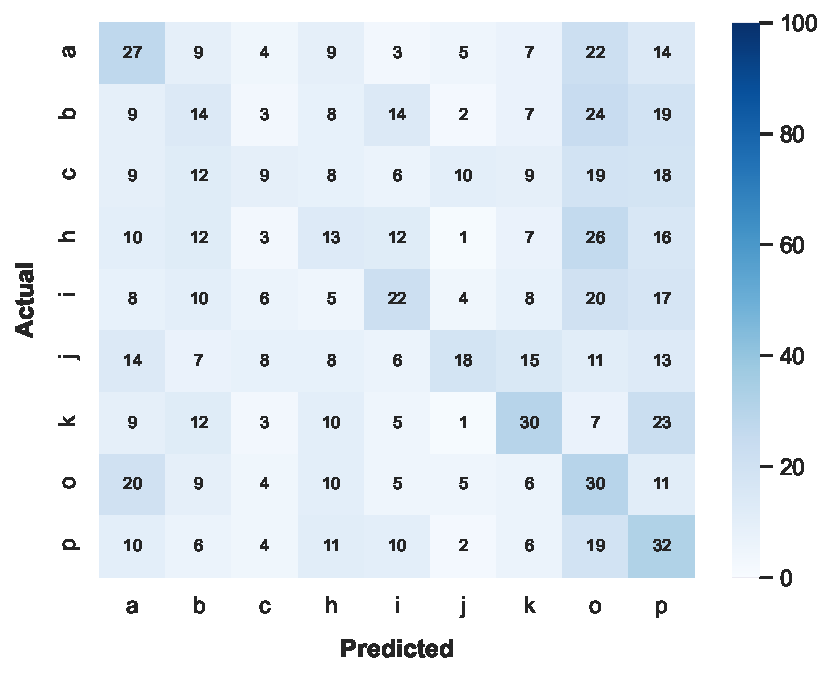
\includegraphics[width=.99\linewidth]{Figures/RadarExperiments/Datasets/ThroughMaterials/PVC+Glass/confusion-filtering-ud.pdf}
      \vspace{-15pt}
      \captionsetup{width=.99\linewidth}
      \caption{Filtering $N{=}20$, \\ $\splitatcommas{AP{=}(1, 2, 3, 6, 8, 9)}$.}
      \label{fig:radar-experiments:through-materials:pvc-glass-confusion:filtering-ud}
  \end{subfigure}
  
  \vspace{-6pt}
  \caption{Normalized confusion matrices for the best configuration at two stages of the pipeline in the user-dependent scenario when using PVC data for training and glass data for testing. The values in each cell are represented as percentages.}
  \label{fig:radar-experiments:through-materials:pvc-glass-confusion}
\end{figure}

% GLASS+PVC
\begin{figure}[ht]
  \begin{subfigure}{.49\textwidth}
    \centering
    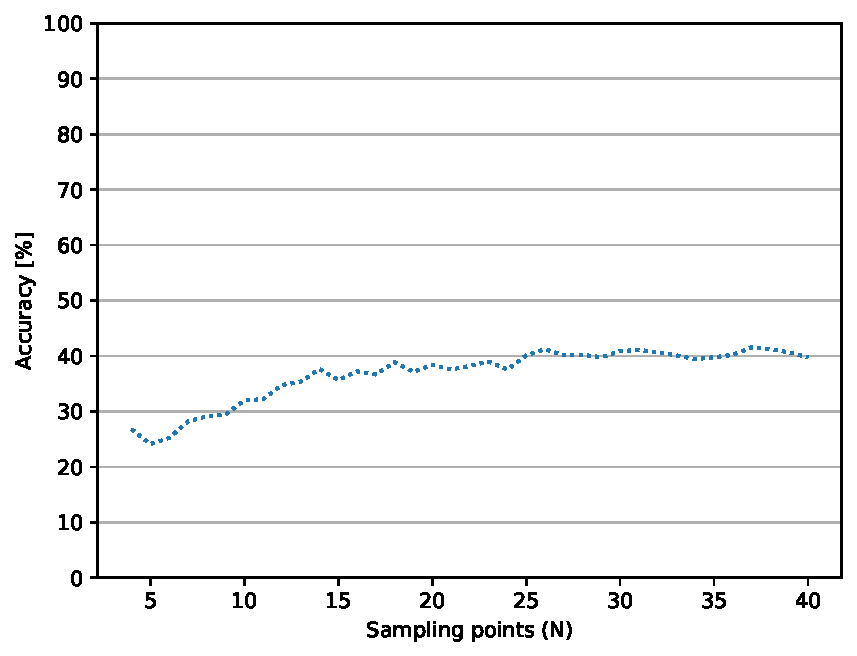
\includegraphics[width=.99\linewidth]{Figures/RadarExperiments/Datasets/ThroughMaterials/Glass+PVC/samples-timegating-ud.pdf}
    \vspace{-15pt}
    \captionsetup{width=.99\linewidth}
    \caption{Time gating \\ $\splitatcommas{AP{=}(4, 5, 7, 10, 11, 12)}$.}
    \label{fig:radar-experiments:through-materials:glass-pvc-samples:timegating-ud}
  \end{subfigure}
  \begin{subfigure}{.49\textwidth}
    \centering
    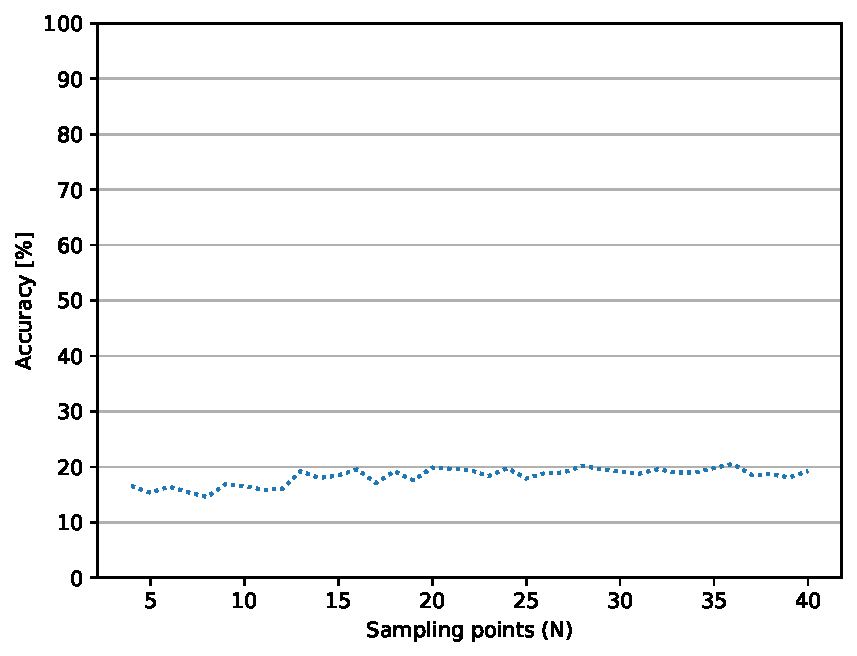
\includegraphics[width=.99\linewidth]{Figures/RadarExperiments/Datasets/ThroughMaterials/Glass+PVC/samples-filtering-ud.pdf}  
    \vspace{-15pt}
    \captionsetup{width=.99\linewidth}
    \caption{Filtering \\ $\splitatcommas{AP{=}(1, 2, 3, 6, 8, 9)}$.}
    \label{fig:radar-experiments:through-materials:glass-pvc-samples:filtering-ud}
  \end{subfigure}

  \vspace{-6pt}
  \caption{The accuracy of Jackknife with respect to the number of sampling points for the best performing set of antenna pairs when using glass data for training and PVC data for testing in a user-dependent scenario.}
  \label{fig:radar-experiments:through-materials:glass-pvc-samples}
\end{figure}

\begin{figure}[ht]
  \begin{subfigure}{.49\textwidth}
      \centering
      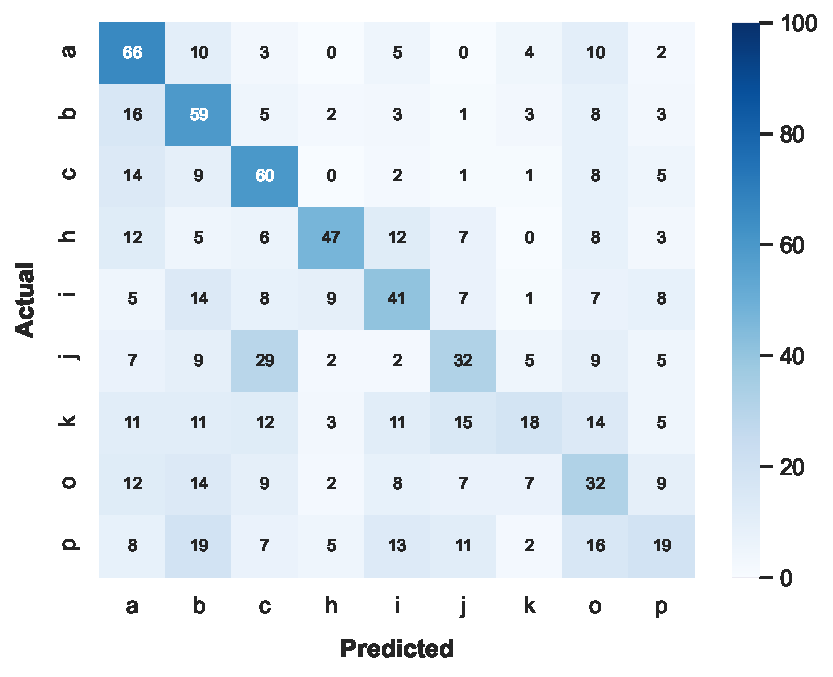
\includegraphics[width=.99\linewidth]{Figures/RadarExperiments/Datasets/ThroughMaterials/Glass+PVC/confusion-timegating-ud.pdf}
      \vspace{-15pt}
      \captionsetup{width=.99\linewidth}
      \caption{Time gating $N{=}37$, \\ $\splitatcommas{AP{=}(4, 5, 7, 10, 11, 12)}$.}
      \label{fig:radar-experiments:through-materials:glass-pvc-confusion:timegating-ud}
  \end{subfigure}
  \begin{subfigure}{.49\textwidth}
      \centering
      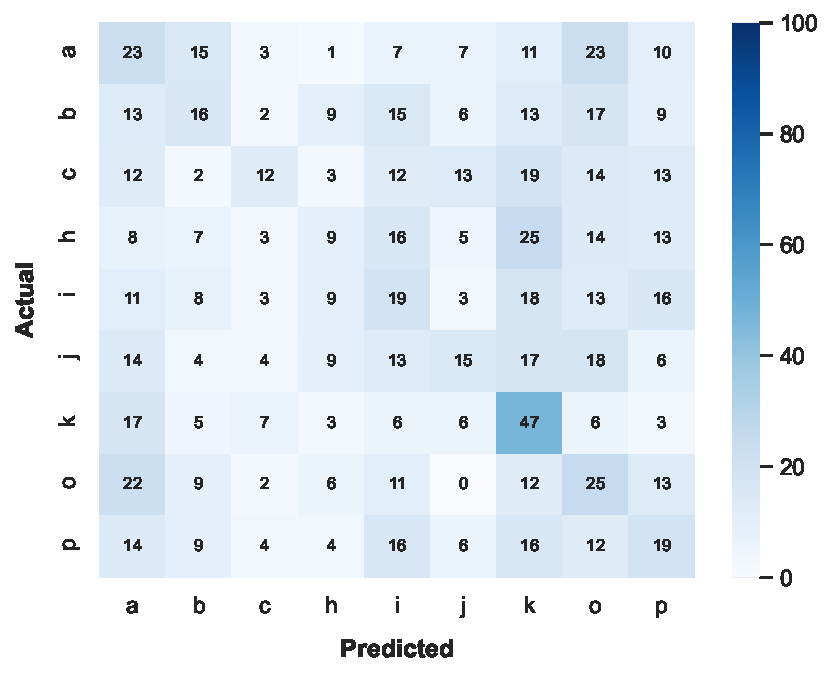
\includegraphics[width=.99\linewidth]{Figures/RadarExperiments/Datasets/ThroughMaterials/Glass+PVC/confusion-filtering-ud.pdf}
      \vspace{-15pt}
      \captionsetup{width=.99\linewidth}
      \caption{Filtering $N{=}36$, \\ $\splitatcommas{AP{=}(1, 2, 3, 6, 8, 9)}$.}
      \label{fig:radar-experiments:through-materials:glass-pvc-confusion:filtering-ud}
  \end{subfigure}
  
  \vspace{-6pt}
  \caption{Normalized confusion matrices for the best configuration at two stages of the pipeline in the user-dependent scenario when using glass data for training and PVC data for testing. The values in each cell are represented as percentages.}
  \label{fig:radar-experiments:through-materials:glass-pvc-confusion}
\end{figure}

